\chapter{Experimental results and conclusions}
\section{Results}
Our propose in a nutshell is a new substitutive method of Watershed transform. The following results are obtained using an Acer Aspire E1 laptop with 8 gb of RAM. The figure \ref{fig:alltheprocess} shows all the process starting from the gray scale image to the mask used to find only the leukocytes.
\begin{figure}[htbp]
    \centering
    \begin{subfigure}[b]{0.45\textwidth}
        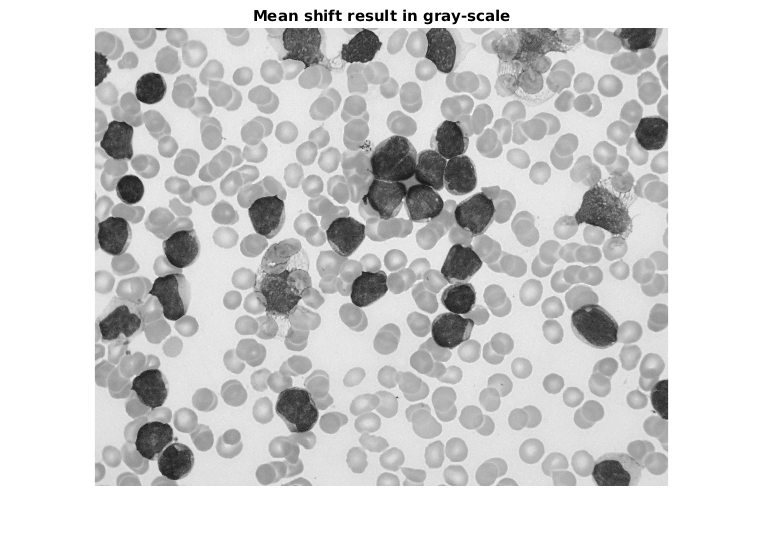
\includegraphics[width=\textwidth]{img/final/figure1.png}
        \caption{ }
        \label{fig:fig1}
    \end{subfigure}
      %(or a blank line to force the subfigure onto a new line)
    \begin{subfigure}[b]{0.45\textwidth}
        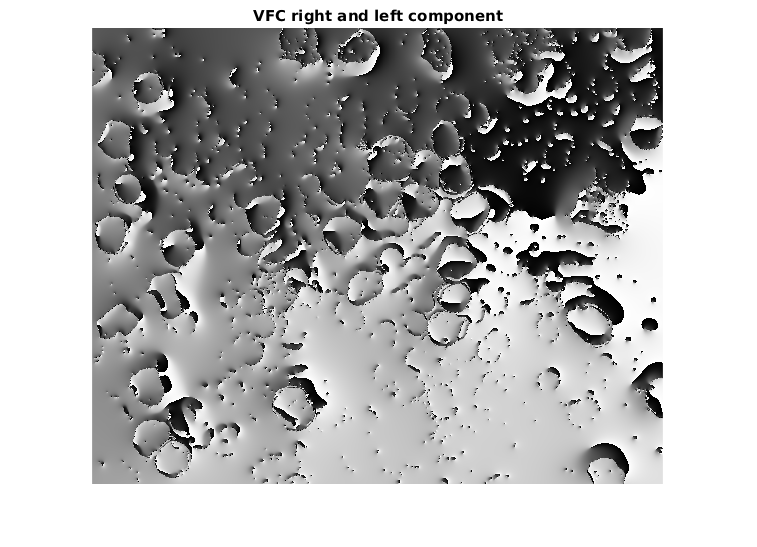
\includegraphics[width=\textwidth]{img/final/figure2.png}
        \caption{ }
        \label{fig:fig}
    \end{subfigure}
    \begin{subfigure}[b]{0.45\textwidth}
        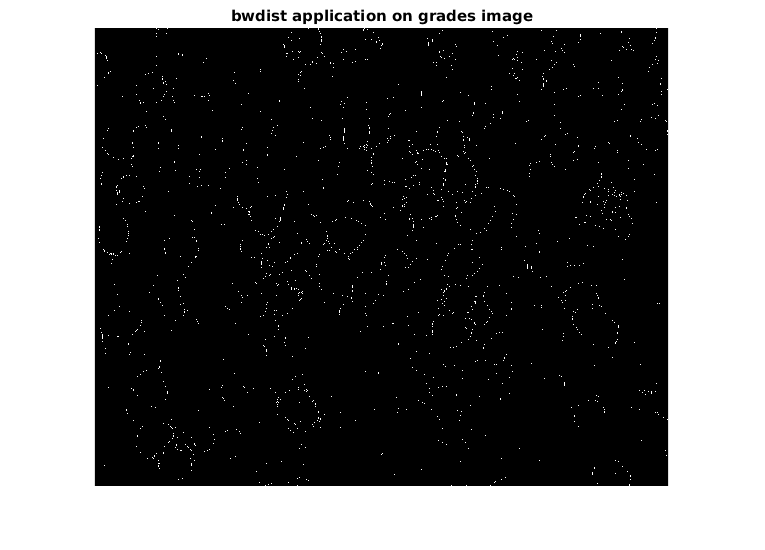
\includegraphics[width=\textwidth]{img/final/figure3.png}
        \caption{ }
        \label{fig:fig3}
    \end{subfigure}
    \begin{subfigure}[b]{0.45\textwidth}
        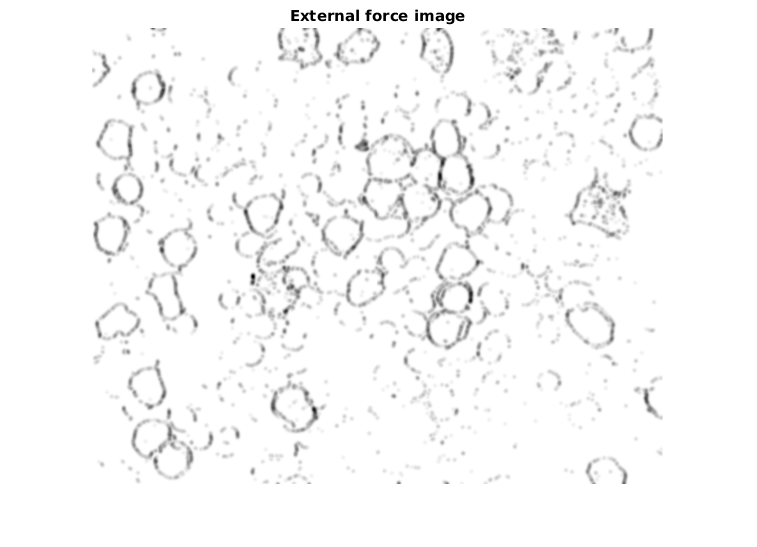
\includegraphics[width=\textwidth]{img/final/figure4.png}
        \caption{ }
        \label{fig:fig4}
    \end{subfigure}
    \begin{subfigure}[b]{0.45\textwidth}
        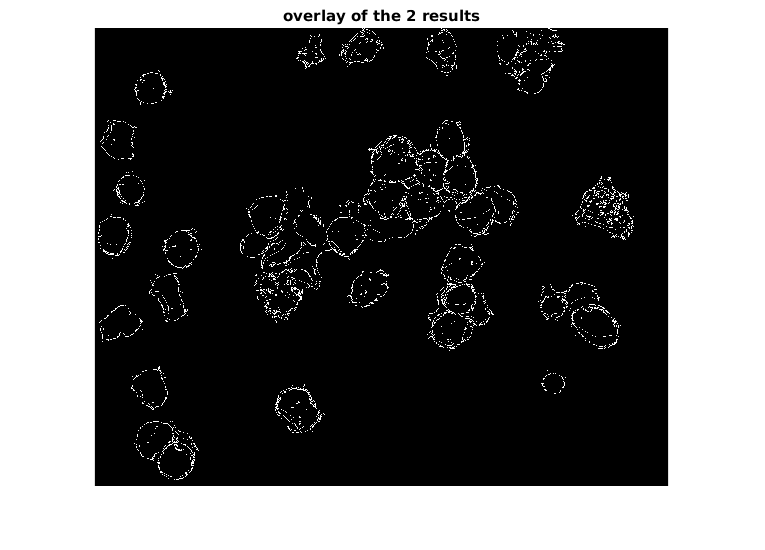
\includegraphics[width=\textwidth]{img/final/figure5.png}
        \caption{ }
        \label{fig:fig5}
    \end{subfigure}
    \begin{subfigure}[b]{0.45\textwidth}
        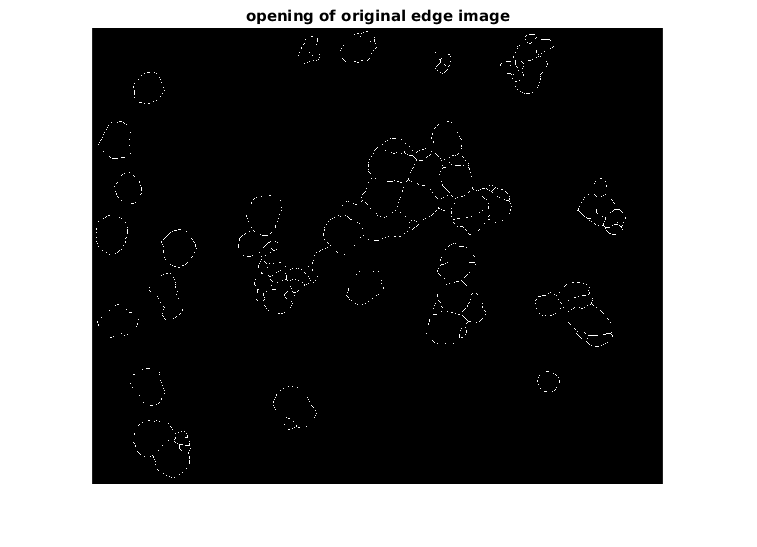
\includegraphics[width=\textwidth]{img/final/figure6.png}
        \caption{ }
        \label{fig:fig6}
    \end{subfigure}
    \begin{subfigure}[b]{0.45\textwidth}
        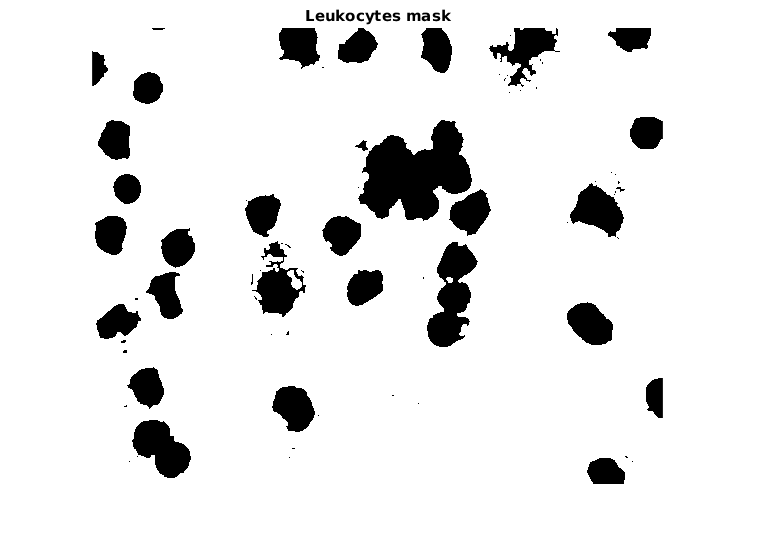
\includegraphics[width=\textwidth]{img/final/figure7.png}
        \caption{ }
        \label{fig:fig7}
    \end{subfigure}

    
    \caption{(a) Mean shift result in gray scale,(b) VFC u and v components,(c) Distance transform on grades image,(d) External force image,(e) Overlay of two results,(f) Opening of initial edge image,(g) Leukocytes mask}
    \label{fig:alltheprocess}
\end{figure}
The last two figures \ref{fig:fig8} \ref{fig:fig9} show the real result of the segmentation.

\begin{figure}
\centering
	\begin{center}
		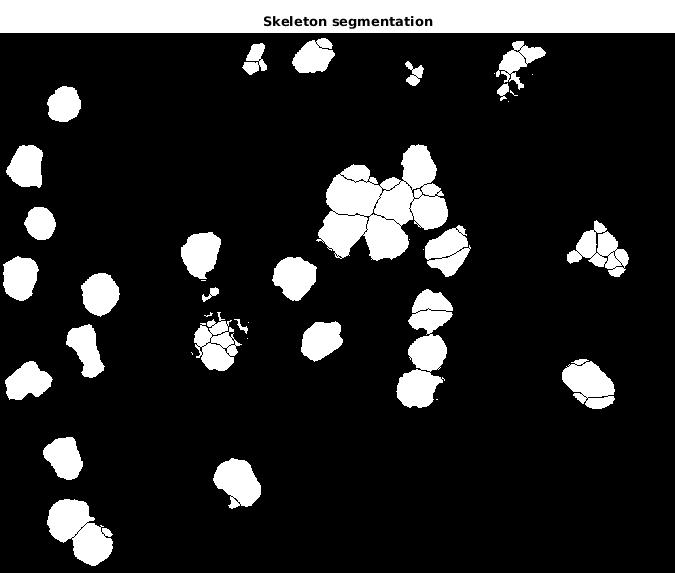
\includegraphics[scale=0.5]{img/final/figure8.png}
		\caption{Skeleton segmentation}
		\label{fig:fig8}
	\end{center}
\end{figure}
\begin{figure}
\centering
	\begin{center}
		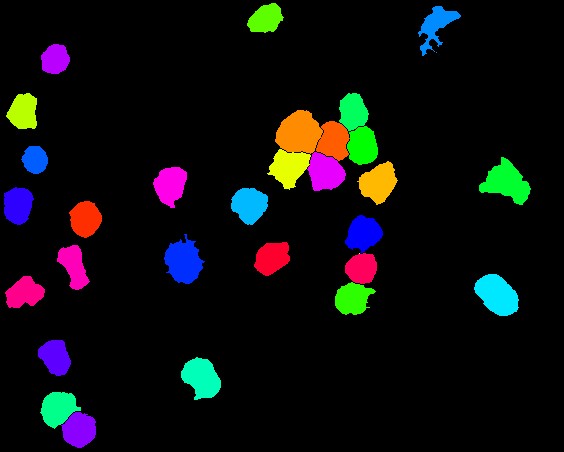
\includegraphics[scale=0.5]{img/final/untitled.png}
		\caption{Merging of little area to count the number of leukocytes}
		\label{fig:fig9}
	\end{center}
\end{figure}
\bigskip
\begin{figure}
\begin{center}
		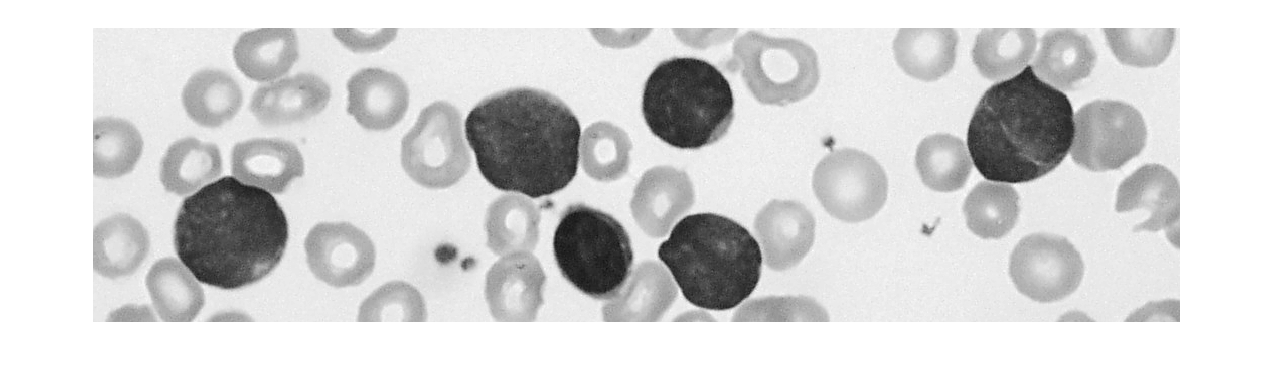
\includegraphics[scale=0.3]{img/final/nooverlap.png}
		\caption{Granulocite after Mean shift application}
		\label{fig:noover}
\end{center}
\end{figure}
\begin{figure}
\begin{center}
		
\includegraphics[scale=0.3]{img/final/nooverlapseg.png}
		\caption{Granulocite after Mean shift application}
		\label{fig:nooverseg}
\end{center}
\end{figure}

As it possible to see, between the two images \ref{fig:fig8} and \ref{fig:fig9} there are some differences. The more visible difference is the bigger presence of agglomerate of small areas that create a kind of cell in the first segmentation. This happened because it was an artefact caused by the Giemsa stain method, but in our approach we can discriminate all this little areas going to remove them because the over-segmentation of this kind (where there are only little areas) means that it is not a leukocyte but only a stain of colour. The result of the counting in this case is 29. 
Working with cropped images we obtain a better result because we have to analyse less cells and as a consequence we have an increase of the speed as it is explained in the table \ref{statistics}.
\begin{table}
\centering
\begin{tabular}{|c|c|c|c|}
\hline 
name & cropped & time & Number of recognized cells / number of real cells\\ 
\hline 
image 5 & no & 45.050214 & 29/29\\ 
\hline 
image 5 & yes & 2.214306 & 7/7\\ 
\hline 
image 13 & no & 31.827737 & 11/11 \\ 
\hline 
image 13 & yes & 1.189616 & 4/4 \\ 
\hline 
image 18 & no & 31.493120 & 18/17\\ 
\hline 
image 18 & yes & 1.717642 & 3/3 \\ 
\hline 
\end{tabular} 
\caption{Statistics result}
\label{statistics}
\end{table}
The table shows only the images where is present the worst case of overlap and clump between the cells. The images where is not present any kind of contact between the cells are well segmented with no problem of over-segmentation with an accuracy of 100\%. In the images  \ref{fig:noover}, \ref{fig:nooverseg} there is an example of segmentation of six cells without any kind of over-segmentation or division. This is only an example but our implementation works very well with all the images with no overlapped cells. In this case we do not need the mean shift application because the cells are well distant from themselves. This means that the computational cost is very less then the version with the mean shift application (total time $<$ 1 second).

\section{Related works}
Checking the results in presence of clumps or cells overlap, our obtained results are better if we compare them with the results of another work that uses the same dataset \cite{otherwork}. In this work the WBC counting is performed by counting a number of connected components but it is not present a method to divide the clumped cells. We obtain a very close result if we compare our system with a previous work proposed in \cite{dirub} even though in this work the clumped and the overlapped cells are not well segmented. To evaluate the results, we compared ours with the results obtained in \cite{water} in term of accuracy. 
\begin{table}
\begin{tabular}{|c|c|c|}
\hline
number image &  accuracy related work (in \%) & accuracy our work (in \%)\\ 
1 &  55 & 100 \\ 
\hline
2 &  100 & 83 \\ 
\hline 
3 &  91 & 100 \\ 
\hline
4 &  57 & 86 \\ 
\hline
5 &  79 & 100 \\ 
\hline
6 &  100 & 86 \\ 
\hline
7 &  100 & 100 \\ 
\hline
8 &  94 & 94 \\ 
\hline
9 &  100 & 100 \\ 
\hline
10 &  100 & 100 \\ 
\hline
11 &  80 & 100 \\ 
\hline
12 &  100 & 94 \\ 
\hline
13 &  70 & 100 \\ 
\hline
14 &  60 & 100 \\ 
\hline
15 &  100 & 100 \\ 
\hline
16 &  100 & 95 \\ 
\hline
17 &  100 & 100 \\ 
\hline
18 &  100 & 93 \\ 
\hline
19 &  100 & 91 \\ 
\hline
20 &  100 & 100 \\ 
\hline
21 &  100 & 100 \\ 
\hline
22 &  100 & 100 \\ 
\hline
23 &  100 & 100 \\ 
\hline
24 &  100 & 100 \\ 
\hline
25 &  100 & 100 \\ 
\hline
26 &  100 & 100 \\ 
\hline
27 &  100 & 100 \\ 
\hline
28 &  100 & 100 \\ 
\hline
29 &  100 & 100 \\ 
\hline
30 &  100 & 100 \\ 
\hline
31 &  100 & 100 \\ 
\hline
32 &  100 & 100 \\ 
\hline
33 &  100 & 100 \\
\hline
\end{tabular} 
\caption{Performance of the proposed method for WBCs identification}
\label{resulttab}
\end{table}
Taking a look on the results showed in table \ref{resulttab} it is evident that our worst score (86\%) is better than the worst result of the related work (55\%). In this case the images are composed of significant overlaps between leukocytes, which are difficult to find even for human experts pathologists.




\section{Conclusions and future works}
The dissertation proposed an innovative white blood cell recognition and segmentation system. It was implemented using some notions already known in literature but never applied in this field. Combining them we obtain a new innovative method in which the major innovation is the use of the Vector field convolution in union to the mean shift and the skeleton function to obtain a result better than the watershed method in terms of cells separation from clumps.

\bigskip

The algorithm produces very good results where we analyse images where granulocytes are missing, because the shape of its nucleus produces a not properly segmentation; however we can use it as a base for a detection system \ref{fig:grangray} \ref{fig:gran}
\begin{figure}
\begin{center}
		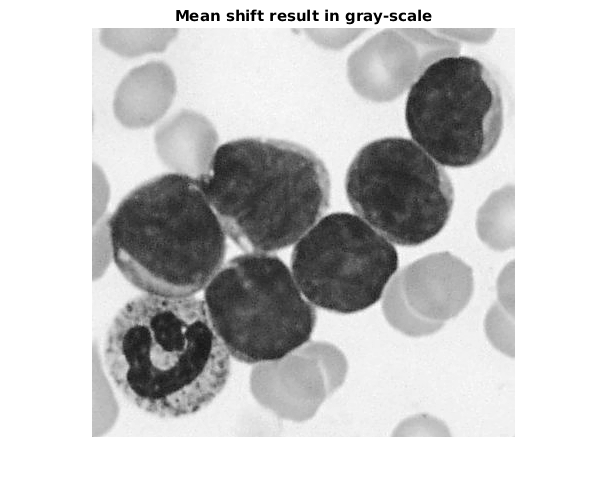
\includegraphics[scale=0.5]{img/final/meangran.png}
		\caption{Granulocite after Mean shift application}
		\label{fig:grangray}
\end{center}
\end{figure}
\begin{figure}
\begin{center}
		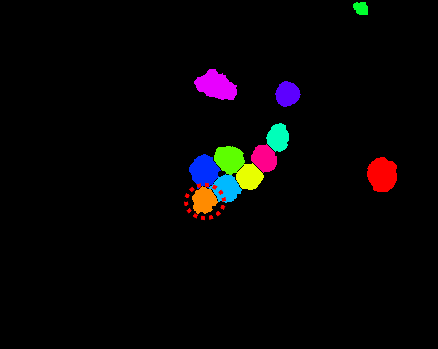
\includegraphics[scale=0.5]{img/final/fingran1.png}
		\caption{Granulocyte segmentation}
		\label{fig:gran}
\end{center}
\end{figure}
The most important points that we focused in this thesis can be listed as follows:
\bigskip

\begin{minipage}{\linewidth}
\begin{enumerate}
\item preprocessing by using the mean shift algorithm in order to reduce all the differences of colour inside the cells;
\item extrapolation of the right and left component of the VFC force;
\item application of the skeleton in order to separate the overlapped cells;
\item recognize and count of the cells.
\end{enumerate}
\end{minipage}

\bigskip

Our method demonstrates that, at this moment, it is better than every algorithm existing in literature. The only remaining issues are that it cannot be too robust, due to the low quality of images and the over-segmentation caused by the granulocytes. But as the literature says, this is the complex field in haematological image segmentation.

\bigskip

Future works will include to propose a new kind of region merging algorithm in order to delete all the over-segmentation,  an improvement to obtain a better segmentation of granulocytes and a new points-linking function to remove the skeleton side of the algorithm and use only the information given by the VFC components.